\subsubsection{Database -- PostgreSQL}
\label{subsubsec:postgresql-database}

The system database is planned on PostgreSQL and stores, in one place, the data
used by both the administrator and the user subsystems. The design aims to support
the functions in the assignment, limit duplicated data and keep related
information consistent.

The planned groups of data are:

\begingroup
\small
\setlength{\tabcolsep}{4pt}
\begin{longtable}{|L{2cm}|L{4cm}|L{3cm}|L{\dimexpr\textwidth-9cm-8\tabcolsep-5\arrayrulewidth\relax}|}
  \caption{Planned data groups and who works with them}
  \label{tab:data-groups}\\
  \hline
  \textbf{Data group} & \textbf{Planned content} &
  \textbf{Purpose} & \textbf{Actor and scope}\\
  \hline
  \endfirsthead
  \hline
  \textbf{Data group} & \textbf{Planned content} &
  \textbf{Purpose} & \textbf{Actor and scope}\\
  \hline
  \endhead
  Accounts &
  Username, hashed password, personal profile, role and account status &
  Sign-in, authorization and user management &
  \textbf{User:} registers, updates their own profile and password.
  \textbf{Admin:} views, adds, updates, deletes, locks/unlocks accounts and updates
  passwords with administrator rights.\\
  \hline
  Friendships &
  Friend requests, their status, friendships and the block list &
  Connecting users and managing their relationships &
  \textbf{User:} sends, accepts/declines requests, unfriends and blocks accounts.
  \textbf{Admin:} views friend lists and friend-count statistics.\\
  \hline
  Conversations and messages &
  Participants, sender, content and time of each message &
  Chat, history, and messages read later when the recipient comes back &
  \textbf{User:} sends, views, searches and deletes history within the allowed scope.
  \textbf{Backend:} checks membership, stores and delivers messages.\\
  \hline
  Chat groups &
  Group name, creation time, members and admin rights in the group &
  Managing groups and group messaging &
  \textbf{User:} creates groups and acts according to their rights.
  \textbf{Group admin:} removes members as the rules allow.
  \textbf{System admin:} views groups, members and group admins.\\
  \hline
  Spam reports &
  Reporter, reported account, related content and time of the report &
  Helping administrators review and act &
  \textbf{User:} sends spam reports.
  \textbf{Admin:} views, filters and sorts reports and locks the reported account.\\
  \hline
  Sign-ins and activity &
  Sign-in history, app opens and data about chat activity &
  Monitoring and statistics over a period &
  \textbf{Backend:} records data from system events.
  \textbf{Admin:} views the history, the activity list and the charts.\\
  \hline
\end{longtable}
\endgroup

``Actor'' means who starts or uses the function. Every PostgreSQL read or write goes
through the backend after an authorization check; Admin and User never access the
database directly.

These data groups are the basis for the tables and relationships; a group does not
necessarily map to one table. The detailed design defines the primary keys, foreign
keys and constraints that prevent duplicate records and invalid references.

For operations that change several related records, the team plans to use
transactions so the changes are applied together. For example, accepting a friend
request updates the request status and records the friendship in the same
transaction.

The backend is planned to access PostgreSQL through DAOs and JDBC. The connection
settings are managed by the backend; the Admin Client and the User Client only
exchange requests and results with the server over TCP sockets.

The logical design below turns the data groups into the planned entities,
attributes, keys and relationships. It is implemented in V1 by
\texttt{script/create\_database.sql}, with shared sample data in
\texttt{script/sample\_data.sql}; connecting the applications to the data belongs
to the next implementation stage.

\paragraph{Entity relationship diagram}
\mbox{}\par

The ERD has 11 entities, grouped into accounts, friendships, conversations and
messages, spam reports, and sign-ins and activity. \texttt{Conversation} is shared
by private conversations and group chats, told apart by the \texttt{type}
attribute. Members and their rights in each conversation are managed through
\texttt{ConversationMember}.

Figure~\ref{fig:erd-chatapp-v1} shows the whole model. The attributes are
described again in Table~\ref{tab:data-dictionary} for easy reference.
In the figure, PK is a primary key, FK a foreign key and UK a unique value;
a question mark marks an attribute that may have no value. The symbols 1 and 0..N
show a one-to-many relationship, where the many side may have no records yet.

\begin{landscape}
\begin{figure}[p]
  \centering
  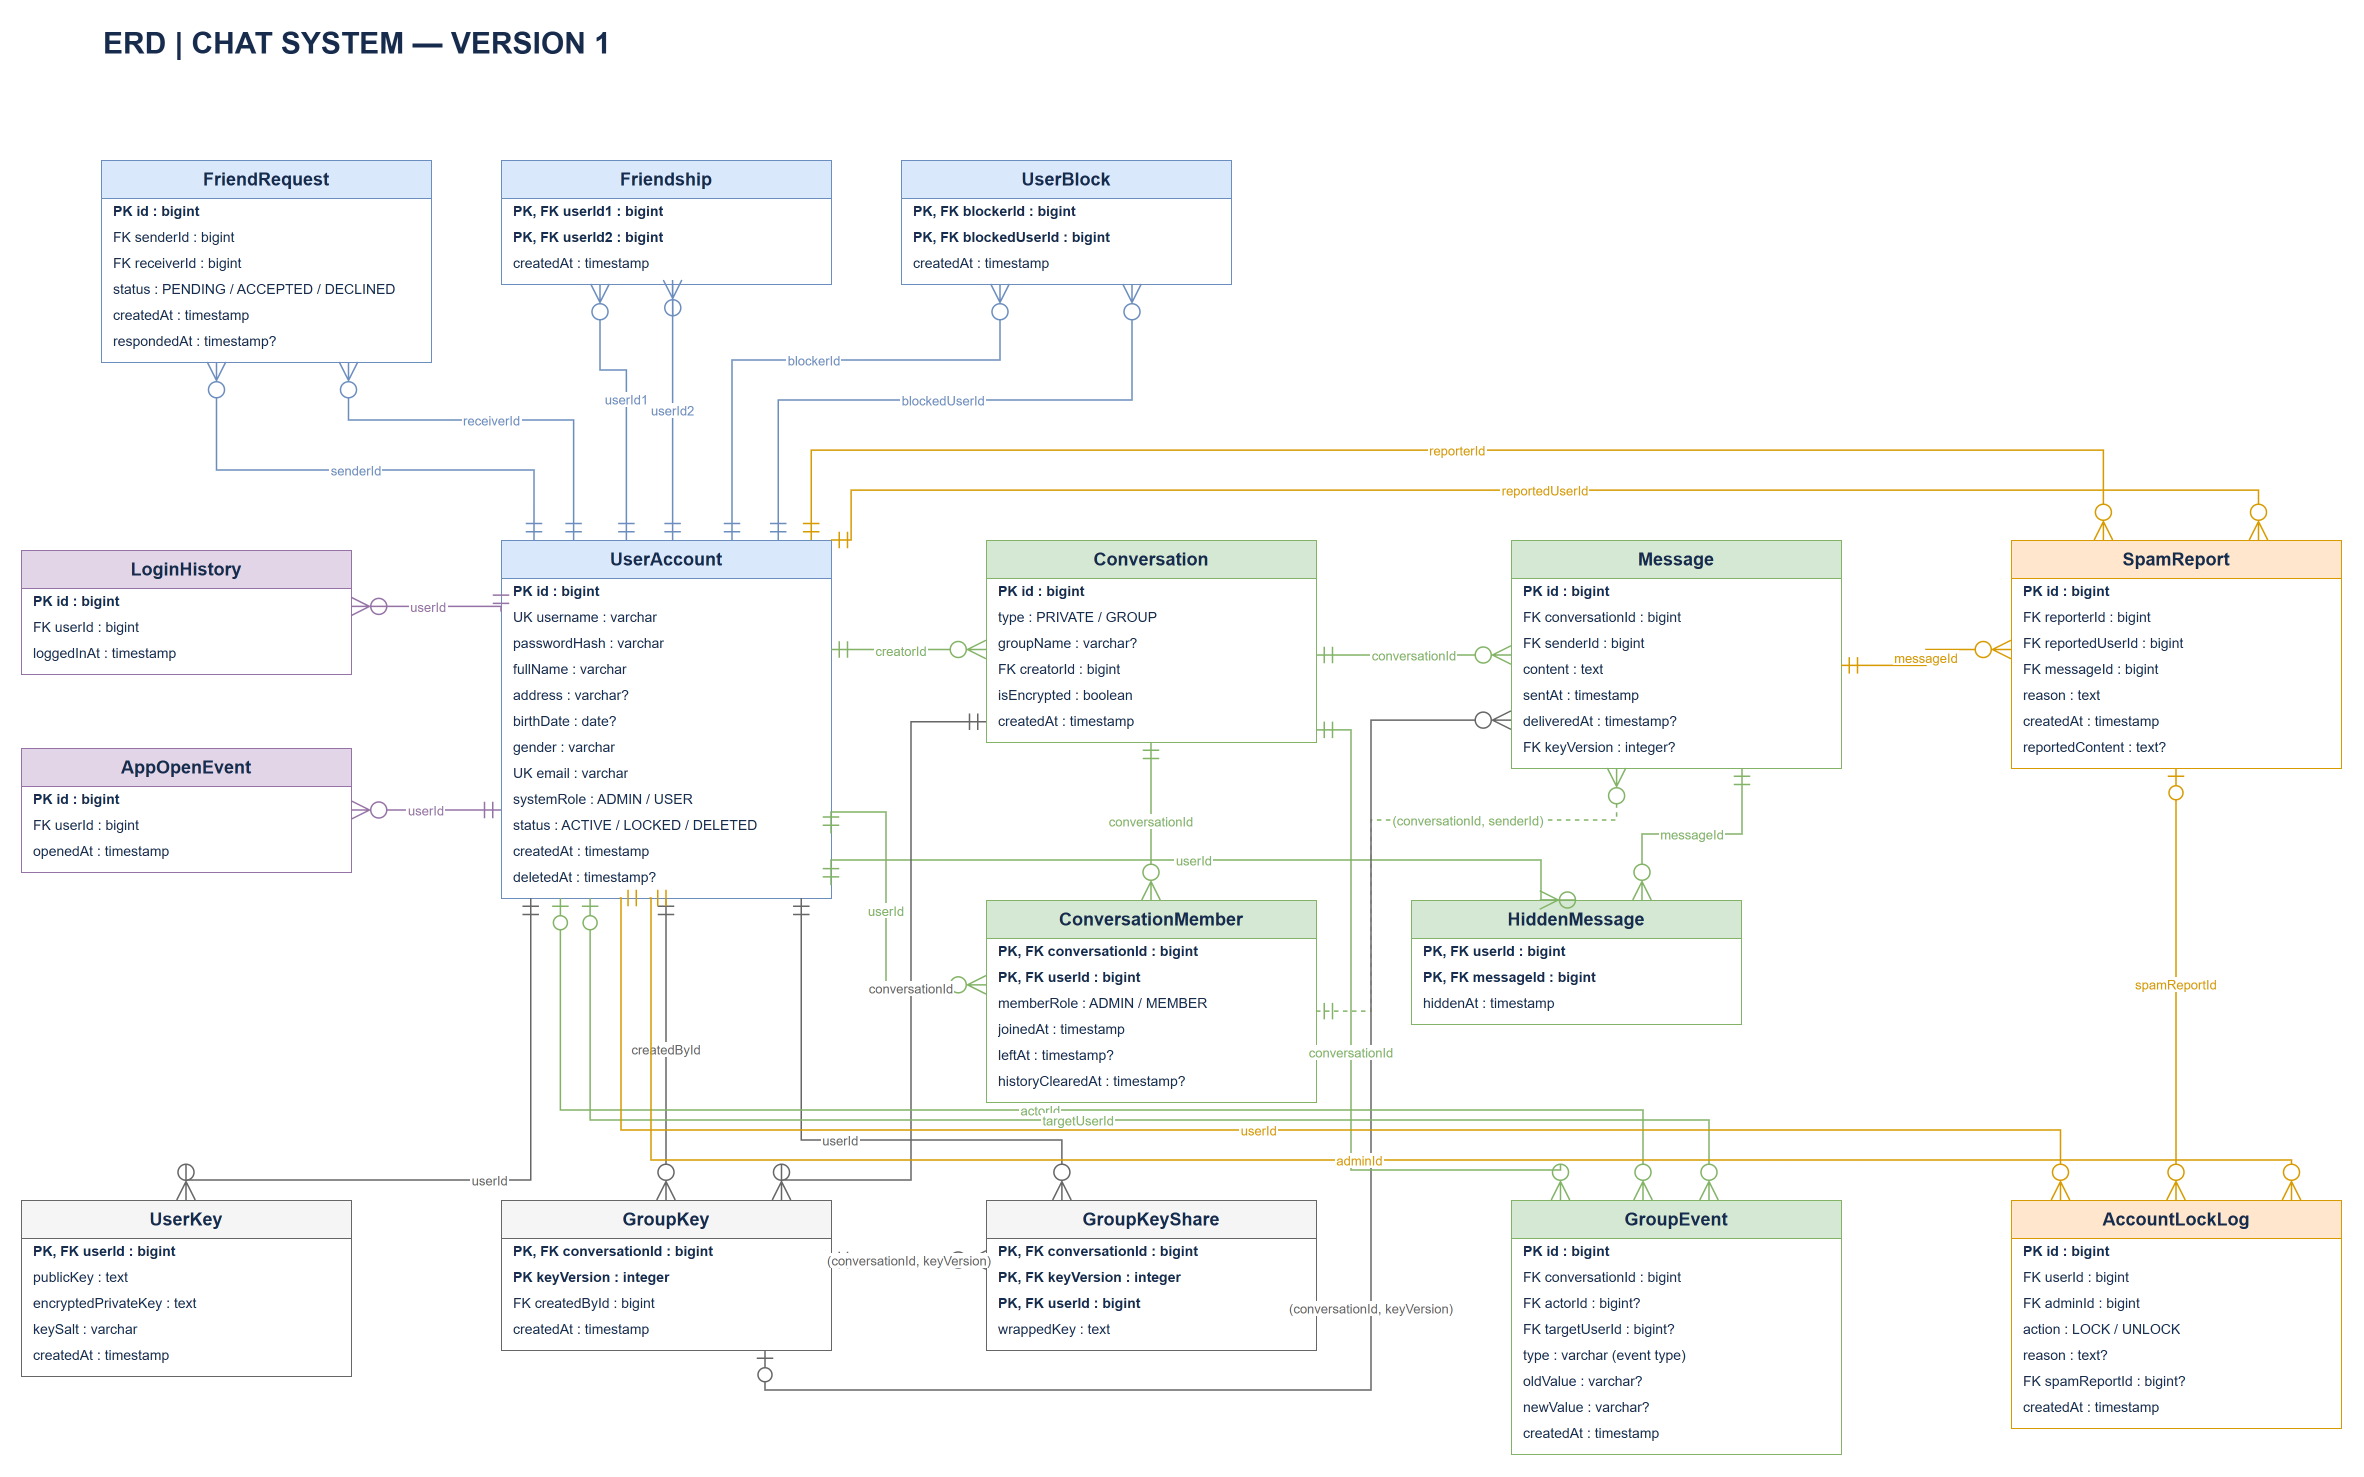
\includegraphics[width=\linewidth,height=0.83\textheight,keepaspectratio]{images/ERD-chatapp-v1.drawio.png}
  \caption{Entity relationship diagram of the chat system.}
  \label{fig:erd-chatapp-v1}
\end{figure}
\end{landscape}

Entity and attribute names in the text match the diagram. Data types in the ERD
are logical; string lengths, default values and the on-delete policy are decided
when the PostgreSQL script is finished.

\paragraph{Data dictionary}
\mbox{}\par

The table below describes the attributes of the 11 entities in the ERD. For a
composite primary key, the attributes marked PK in the same entity form one key
together; each attribute on its own does not have to be unique. Attributes without
a question mark in the figure are expected to have a value; fields that may be
empty are noted in the key and nullability column.

\begingroup
\small
\setlength{\tabcolsep}{4pt}
\begin{longtable}{|L{3.6cm}|L{1.8cm}|L{2.9cm}|L{\dimexpr\textwidth-8.3cm-8\tabcolsep-5\arrayrulewidth\relax}|}
  \caption{Entities and attributes of the database design}
  \label{tab:data-dictionary}\\
  \hline
  \textbf{Attribute} & \textbf{Logical type} & \textbf{Key and nullability} & \textbf{Meaning}\\
  \hline
  \endfirsthead
  \hline
  \textbf{Attribute} & \textbf{Logical type} & \textbf{Key and nullability} & \textbf{Meaning}\\
  \hline
  \endhead
  \multicolumn{4}{|l|}{\textbf{UserAccount}}\\*
  \hline
  \texttt{id} & \texttt{bigint} & PK; Required & Account identifier.\\
  \hline
  \texttt{username} & \texttt{varchar} & UK; Required & Unique username; the upper/lower case rule is decided when the database is created.\\
  \hline
  \texttt{passwordHash} & \texttt{varchar} & Required & Password hash; passwords are never stored as plain text.\\
  \hline
  \texttt{fullName} & \texttt{varchar} & Required & The user's full name.\\
  \hline
  \texttt{address} & \texttt{varchar} & Nullable & Address in the personal profile.\\
  \hline
  \texttt{birthDate} & \texttt{date} & Nullable & Date of birth, separate from activity timestamps.\\
  \hline
  \texttt{gender} & \texttt{varchar} & Required & Gender in the personal profile.\\
  \hline
  \texttt{email} & \texttt{varchar} & UK; Required & Unique email, used for contact and password reset.\\
  \hline
  \texttt{systemRole} & \texttt{varchar} & Required & System role: \texttt{ADMIN} or \texttt{USER}.\\
  \hline
  \texttt{status} & \texttt{varchar} & Required & Account status: \texttt{ACTIVE} or \texttt{LOCKED}.\\
  \hline
  \texttt{createdAt} & \texttt{timestamp} & Required & When the account was created; used for new-registration statistics.\\
  \hline
  \multicolumn{4}{|l|}{\textbf{FriendRequest}}\\*
  \hline
  \texttt{id} & \texttt{bigint} & PK; Required & Friend request identifier.\\
  \hline
  \texttt{senderId} & \texttt{bigint} & FK; Required & Account that sent the request, references \texttt{UserAccount.id}.\\
  \hline
  \texttt{receiverId} & \texttt{bigint} & FK; Required & Account that received the request, references \texttt{UserAccount.id}.\\
  \hline
  \texttt{status} & \texttt{varchar} & Required & Status \texttt{PENDING}, \texttt{ACCEPTED} or \texttt{DECLINED}.\\
  \hline
  \texttt{createdAt} & \texttt{timestamp} & Required & When the request was sent.\\
  \hline
  \texttt{respondedAt} & \texttt{timestamp} & Nullable & When it was accepted or declined; empty while pending.\\
  \hline
  \multicolumn{4}{|l|}{\textbf{Friendship}}\\*
  \hline
  \texttt{userId1} & \texttt{bigint} & Composite PK, FK; Required & First account; references \texttt{UserAccount.id}.\\
  \hline
  \texttt{userId2} & \texttt{bigint} & Composite PK, FK; Required & Second account; references \texttt{UserAccount.id}.\\
  \hline
  \texttt{createdAt} & \texttt{timestamp} & Required & When the friendship started.\\
  \hline
  \multicolumn{4}{|l|}{\textbf{UserBlock}}\\*
  \hline
  \texttt{blockerId} & \texttt{bigint} & Composite PK, FK; Required & Account that blocks, references \texttt{UserAccount.id}.\\
  \hline
  \texttt{blockedUserId} & \texttt{bigint} & Composite PK, FK; Required & Account that is blocked, references \texttt{UserAccount.id}.\\
  \hline
  \texttt{createdAt} & \texttt{timestamp} & Required & When the block was created.\\
  \hline
  \multicolumn{4}{|l|}{\textbf{Conversation}}\\*
  \hline
  \texttt{id} & \texttt{bigint} & PK; Required & Conversation identifier.\\
  \hline
  \texttt{type} & \texttt{varchar} & Required & Conversation type: \texttt{PRIVATE} or \texttt{GROUP}.\\
  \hline
  \texttt{groupName} & \texttt{varchar} & Nullable & Group name; not used for private conversations.\\
  \hline
  \texttt{creatorId} & \texttt{bigint} & FK; Required & Account that created the conversation, references \texttt{UserAccount.id}.\\
  \hline
  \texttt{isEncrypted} & \texttt{boolean} & Required & Flag for an encrypted group; it does not replace key management data.\\
  \hline
  \texttt{createdAt} & \texttt{timestamp} & Required & When the conversation or group was created.\\
  \hline
  \multicolumn{4}{|l|}{\textbf{ConversationMember}}\\*
  \hline
  \texttt{conversationId} & \texttt{bigint} & Composite PK, FK; Required & Conversation joined, references \texttt{Conversation.id}.\\
  \hline
  \texttt{userId} & \texttt{bigint} & Composite PK, FK; Required & Participant, references \texttt{UserAccount.id}.\\
  \hline
  \texttt{memberRole} & \texttt{varchar} & Required & Role in the conversation: \texttt{ADMIN} or \texttt{MEMBER}; separate from the system role.\\
  \hline
  \texttt{joinedAt} & \texttt{timestamp} & Required & When the member joined the conversation.\\
  \hline
  \texttt{leftAt} & \texttt{timestamp} & Nullable & When the member left or was removed from the group; empty while still a member.\\
  \hline
  \texttt{historyClearedAt} & \texttt{timestamp} & Nullable & Point before which the whole history is hidden for this member, since clearing history affects only that person.\\
  \hline
  \multicolumn{4}{|l|}{\textbf{Message}}\\*
  \hline
  \texttt{id} & \texttt{bigint} & PK; Required & Message identifier.\\
  \hline
  \texttt{conversationId} & \texttt{bigint} & FK; Required & Conversation of the message, references \texttt{Conversation.id}; also part of the sender's composite foreign key.\\
  \hline
  \texttt{senderId} & \texttt{bigint} & FK; Required & Sender; with \texttt{conversationId} it references the key of \texttt{ConversationMember}.\\
  \hline
  \texttt{content} & \texttt{text} & Required & Message content. How encrypted content is stored still needs to be designed.\\
  \hline
  \texttt{sentAt} & \texttt{timestamp} & Required & When the message was sent; used to order the history and filter by time.\\
  \hline
  \texttt{deliveredAt} & \texttt{timestamp} & Nullable & When a private message reached its recipient: equal to
  \texttt{sentAt} if the recipient was online, or the time they next signed in if it had to wait; empty while waiting
  and for group messages.\\
  \hline
  \multicolumn{4}{|l|}{\textbf{HiddenMessage}}\\*
  \hline
  \texttt{userId} & \texttt{bigint} & Composite PK, FK; Required & User who hid the message, references \texttt{UserAccount.id}.\\
  \hline
  \texttt{messageId} & \texttt{bigint} & Composite PK, FK; Required & Hidden message, references \texttt{Message.id}.\\
  \hline
  \texttt{hiddenAt} & \texttt{timestamp} & Required & When the user hid the message from their history.\\
  \hline
  \multicolumn{4}{|l|}{\textbf{SpamReport}}\\*
  \hline
  \texttt{id} & \texttt{bigint} & PK; Required & Spam report identifier.\\
  \hline
  \texttt{reporterId} & \texttt{bigint} & FK; Required & Reporting account, references \texttt{UserAccount.id}.\\
  \hline
  \texttt{reportedUserId} & \texttt{bigint} & FK; Required & Reported account, references \texttt{UserAccount.id}.\\
  \hline
  \texttt{messageId} & \texttt{bigint} & FK; Required & Related message, references \texttt{Message.id}.\\
  \hline
  \texttt{reason} & \texttt{text} & Required & Reason or description of the report.\\
  \hline
  \texttt{createdAt} & \texttt{timestamp} & Required & When the report was sent; used for filtering and sorting.\\
  \hline
  \multicolumn{4}{|l|}{\textbf{LoginHistory}}\\*
  \hline
  \texttt{id} & \texttt{bigint} & PK; Required & Sign-in identifier.\\
  \hline
  \texttt{userId} & \texttt{bigint} & FK; Required & Account that signed in, references \texttt{UserAccount.id}.\\
  \hline
  \texttt{loggedInAt} & \texttt{timestamp} & Required & Time of the successful sign-in.\\
  \hline
  \multicolumn{4}{|l|}{\textbf{AppOpenEvent}}\\*
  \hline
  \texttt{id} & \texttt{bigint} & PK; Required & App-open identifier.\\
  \hline
  \texttt{userId} & \texttt{bigint} & FK; Required & Account whose activity is recorded, references \texttt{UserAccount.id}.\\
  \hline
  \texttt{openedAt} & \texttt{timestamp} & Required & When the app was opened; used for app-open and active-user statistics.\\
  \hline
\end{longtable}
\endgroup

Timestamps used for sorting and statistics must be stored and interpreted in one
consistent time zone when the script and the JDBC connection are created. Usernames,
emails, account status and request status also need consistent value conventions.

\paragraph{Main relationships}
\mbox{}\par

An account can send or receive many friend requests, appear in many friendships
and blocks, and take part in many conversations. Where a relationship has two
roles, two attributes reference \texttt{UserAccount.id} with different meanings,
for example the sender and the receiver of a friend request.

\begin{itemize}
  \item \textbf{Accounts and friendships:}
    \texttt{FriendRequest.senderId} and \texttt{receiverId},
    the two attributes of the \texttt{Friendship} primary key,
    and \texttt{UserBlock.blockerId} and \texttt{blockedUserId}
    all reference the matching account.
  \item \textbf{Accounts and conversations:}
    \texttt{Conversation.creatorId} references the creator.
    The many-to-many relationship between accounts and conversations is
    resolved through \texttt{ConversationMember}, whose composite primary key is
    \texttt{(conversationId, userId)}.
  \item \textbf{Conversations and messages:}
    every message belongs to one conversation. The pair
    \texttt{(conversationId, senderId)} in \texttt{Message}
    references the primary key of \texttt{ConversationMember}, which ensures
    the sender has a membership record in that conversation.
    Whether the sender is still a member when sending is checked by the backend.
  \item \textbf{Messages and personal history:}
    \texttt{HiddenMessage} links a user to a message.
    The composite primary key \texttt{(userId, messageId)} prevents recording
    the same hidden message twice for that user.
  \item \textbf{Messages and spam reports:}
    \texttt{SpamReport} references the reporter, the reported account
    and the related message; a message can appear in several reports.
  \item \textbf{Accounts and activity:}
    each \texttt{LoginHistory} or \texttt{AppOpenEvent} record
    belongs to one account; an account can have many records over time.
  \item \textbf{Encryption keys:}
    each account has at most one \texttt{UserKey}. A group has many
    \texttt{GroupKey} versions, keyed by \texttt{(conversationId, keyVersion)};
    each version has one \texttt{GroupKeyShare} per member who may read it.
    \texttt{Message.(conversationId, keyVersion)} references the key version
    used to encrypt the message.
  \item \textbf{Group events:}
    a group has many \texttt{GroupEvent} records; \texttt{actorId} and
    \texttt{targetUserId} reference the accounts involved.
  \item \textbf{Account locks:}
    \texttt{AccountLockLog} references the affected account, the acting
    administrator and, optionally, the \texttt{SpamReport} that led to the lock.
\end{itemize}

\paragraph{Planned constraints and data rules}
\mbox{}\par

Primary keys, foreign keys, unique constraints and \texttt{CHECK} constraints are
implemented in \texttt{script/create\_database.sql}; for example, a message's sender
must be a member of its conversation, a key share can only go to a member, and a
spam report must point to a message written by the reported account.
Rules about access rights, membership status or changing several records at once
are also checked by the backend; the keys in the ERD alone are not enough for
the whole business logic.

\begin{enumerate}
  \item \textbf{Accounts:} the username and email are unique;
    passwords are stored only as hashes. \texttt{systemRole} separates
    system Admins from Users; \texttt{status} separates active accounts
    from locked ones.
  \item \textbf{Friends and blocks:} the two people in a relationship must differ.
    \texttt{Friendship} stores the ID pair with the convention
    \texttt{userId1 < userId2}, combined with the composite primary key so both
    directions of the same relationship are never stored. A block is directed:
    A blocking B does not mean B blocks A.
  \item \textbf{Conversations and members:} \texttt{type} is
    \texttt{PRIVATE} or \texttt{GROUP}; the group name is used for group conversations.
    A private conversation has two participants; creating a group needs the creator
    and at least one other user. The composite primary key of a member prevents
    the same person from appearing twice in a conversation.
  \item \textbf{Group rights:} \texttt{memberRole} is
    \texttt{ADMIN} or \texttt{MEMBER}, independent of system administrator rights.
    Only group admins can remove members, as the assignment requires. On removal the
    backend sets \texttt{leftAt} instead of deleting the \texttt{ConversationMember}
    row, so the composite foreign key of \texttt{Message} stays valid and the person's
    earlier messages remain; when that person is added again, the same row is reused
    and \texttt{leftAt} is cleared.
    When a message is sent, the backend checks the current membership and rights.
  \item \textbf{Locked accounts:} when \texttt{UserAccount.status} is \texttt{LOCKED},
    nobody can message the account privately, send it or accept its friend requests,
    block it, add it to a group or make it a group admin; others can only unfriend it,
    decline its friend requests and, as group admins, remove it from a group.
  \item \textbf{Message status:} the \textbf{Sent}, \textbf{Waiting} and
    \textbf{Delivered} status of a private message is derived from
    \texttt{Message.deliveredAt}, with no extra status column; group messages only
    show \textbf{Sent}.
  \item \textbf{Spam reports:} the reporter must be allowed to see the related
    content; the reported message must belong to the reported account.
    The backend checks these conditions on top of the foreign keys.
  \item \textbf{Encryption and logs:} a key share can only go to someone with a
    membership record in the group, and a message can only name a key version of
    its own conversation (foreign keys); the backend also ensures that keys exist
    only for group conversations, that \texttt{Message.keyVersion} stays empty in
    private conversations and that a new key version is shared only with current
    members. \texttt{AccountLockLog.action} is \texttt{LOCK} or \texttt{UNLOCK},
    \texttt{GroupEvent.type} takes only the listed values, and a user can report
    the same message only once (check and unique constraints).
  \item \textbf{Consistency:} accepting a friend request updates the request and
    creates the friendship in the same transaction. Blocking and unfriending also
    apply their related changes together to avoid contradictory states.
\end{enumerate}

\paragraph{Clearing history and group encryption}
\mbox{}\par

The proposed design treats clearing history as removing it for the person who does
it. \texttt{HiddenMessage} records each hidden message;
\texttt{ConversationMember.historyClearedAt} marks the point before which the whole
history is cleared for that member. When messages are read, hidden messages and
messages before that point are not shown to that person; other participants keep
their history. The team confirms this interpretation when the design is finalised.

Group encryption follows the end-to-end model of encrypted group chats in
Facebook Messenger~\cite{ref:messenger-e2ee}: the server stores and forwards only ciphertext and never
holds a group key in plain form.

\begin{enumerate}
  \item \textbf{User keys:} at registration the client creates an RSA key pair~\cite{ref:rfc8017}.
    The public key is stored in \texttt{UserKey.publicKey}; the private key is
    encrypted on the client with a key derived from the password (PBKDF2~\cite{ref:rfc8018} with
    \texttt{keySalt}), so the user can sign in from any computer.
  \item \textbf{Turning encryption on:} the client of a group admin creates a
    random AES-256 group key (version 1), wraps it with every member's public key
    and uploads one \texttt{GroupKeyShare} per member;
    \texttt{Conversation.isEncrypted} becomes true.
  \item \textbf{Sending and reading:} the sender encrypts the text with the latest
    key version (AES-GCM~\cite{ref:nist-gcm}, a new IV per message) and stores the version in
    \texttt{Message.keyVersion}; members unwrap the matching share with their
    private key to decrypt.
  \item \textbf{Membership changes:} a new member receives a share of the current
    version. When a member leaves or is removed, an admin's client creates a new
    version and shares it only with the remaining members, so the former member
    cannot read later messages.
  \item \textbf{Turning encryption off:} new messages are stored as plain text with
    an empty \texttt{keyVersion}; earlier messages stay encrypted.
\end{enumerate}

Because the server cannot read encrypted messages, searching them is done on the
client after decryption, the AI assistant is not available in encrypted groups,
and a spam report on an encrypted message carries a plain-text copy in
\texttt{SpamReport.reportedContent} sent by the reporter. Changing a password only
re-encrypts the private key. A password reset (a random password sent by email)
cannot recover the old private key: the user receives a new key pair and can read
older encrypted history again only after a group admin shares the keys with the
new public key.

Deleting an account is a soft delete: the administrator's action sets
\texttt{status} to \texttt{DELETED} and records \texttt{deletedAt}, and no row is
removed. Messages, group history, spam reports and lock history therefore stay
complete, every foreign key to \texttt{UserAccount} rejects physical deletion, and a
deleted account can no longer sign in or be found. Its username and email may be
registered again, because uniqueness only applies to accounts that are not deleted.

\paragraph{Data for statistics}
\mbox{}\par

The model has no separate statistics tables when the figures can be computed from
the source data. The Admin functions map as follows:

\begin{itemize}
  \item \hyperlink{F14}{F14}: reads sign-ins from
    \texttt{LoginHistory}, joins the account profile and sorts by time.
  \item \hyperlink{F17}{F17}--\hyperlink{F18}{F18}: filters
    \texttt{UserAccount.createdAt} by the selected year; counts new accounts
    per month of that year.
  \item \hyperlink{F19}{F19}: counts relationships in \texttt{Friendship};
    \textbf{Total network} is the union of direct friends and friends of friends,
    excluding the account itself and counting each account once.
    \textbf{Friends of friends only} also excludes direct friends; a mutual friend
    is found through two consecutive friendships.
  \item \hyperlink{F20}{F20}: counts app opens from
    \texttt{AppOpenEvent}; checks messages, conversations and members to find
    how many people and groups were chatted with in the selected year.
  \item \hyperlink{F21}{F21}: counts distinct accounts that opened the app in
    each month, not the total number of opens.
\end{itemize}

Sign-in history and app opens are kept apart because reopening the app is not
necessarily a new sign-in. Online/offline status will be determined by the backend
from live connections; an old sign-in record does not prove a user is online.

The \textbf{Period} picker applies one calendar year to tables and charts.
A yearly query covers the start of the year up to the start of the next year in the
system's time zone. Charts always show 12 months; the yearly total of
\textbf{Active users} counts each account once, even when it was active in several
months.

\paragraph{Data for administration extensions}
\mbox{}\par
\texttt{UserAccount.status} holds the current \texttt{ACTIVE}/\texttt{LOCKED}
state, and \texttt{AccountLockLog} keeps its history: each lock or unlock records
the account, the administrator, the time and, when it comes from the spam report
screen, the report. The \textbf{Prior locks} count and the \textbf{Admin lock
history} on the Spam Reports screen read from this table. The backend checks that
\texttt{adminId} belongs to an account with \texttt{systemRole = ADMIN} and
updates the status and the log in one transaction.

The \textbf{Activity} and \textbf{Monitoring} tabs of Chat Groups combine two
sources. Message rows come from \texttt{Message} (an encrypted message is shown
only as ``sent an encrypted message''). Every other change is a
\texttt{GroupEvent} written by the backend in the same transaction as the change
itself: creating the group, renaming it, adding a member, a member leaving or
being removed, a role change, and turning encryption on or off.
\texttt{ConversationMember} alone cannot provide this, because it keeps one row per
member, cannot tell leaving from being removed, and overwrites \texttt{joinedAt}
when a member is added again.

